\chapter{UML Profil auf M2 Ebene}
\label{UMLProfil}
In diesem Projekt wurde vorab entschieden, den bestehenden Sprachumfang der UML durch UML-Profile zu erweitern. Ein UML-Profil ist genau genommen eine Erweiterung dessen Metamodells und somit des Standard Sprachumfangs der UML und es ist gleichzeitig ein UML-Modell.

Das UML Profil wird mit eigens definierten Meta Klassen erweitert. Grund hierfür ist, dass im späteren UML Modell Zuständigkeiten besser zugewiesen und erkannt werden können.
Diese Erweiterungen werden als Stereotype im Profil bezeichnet, die von vordefinierten Metaklassen abgeleitet werden.

Im folgenden is die Endfassung des Profils zu sehen, welche anschließend genauer erläutert wird.
\begin{figure}[htbp]
\begin{center}
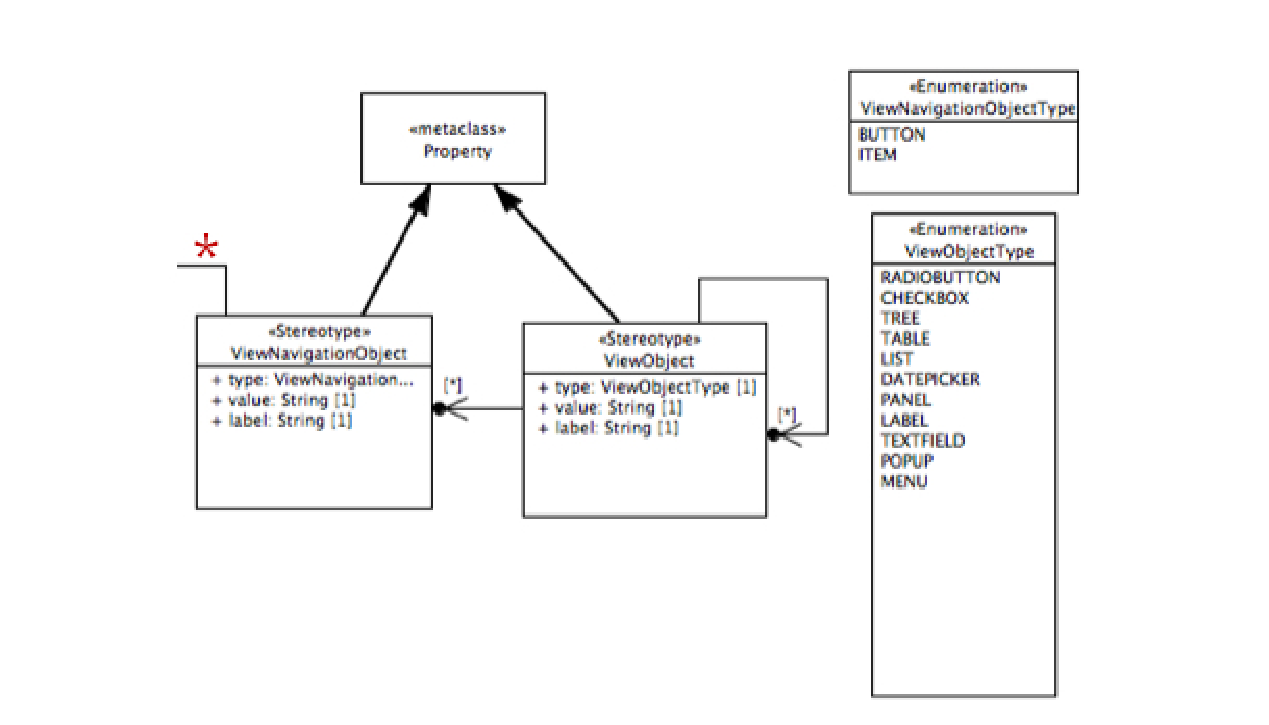
\includegraphics[width=\textwidth]{./img/ProfilProp.pdf}
\caption{Darstellung der Properties und Enumerations im Profil}\label{Fig:UMLProfil}
\end{center}
\end{figure}\\
In dem Profil wurden zwei Stereotypen für Properties definiert. Die \textbf{ViewObject} und die \textbf{ViewNavigationObject}, die die Widgets in GWT repräsentieren. Durch die Frontendbetrachtung gibt es nur Elemente, die entweder zum Anzeigen von Informationen ( \textbf{ViewObject}) oder zum Navigieren auf andere Views (ViewNavigationObject) dienen. Die Trennung der doch ziemlich ähnlichen Elemente musste erfolgen, da es nur so möglich wurde, dass zwar  \textbf{ViewObjects} andere  \textbf{ViewObjects} oder  \textbf{ViewNavigationObjects} enthalten können, bei  \textbf{ViewNavigationObjects} dies wiederum aber nicht möglich sein darf. 
Im Sinne einer besseren Übersichtlichkeit wurde sich darauf geeinigt, den Typ der Property mit Hilfe von Enumerations festzulegen. Diese ermöglichen eine Reduzierung der unterschiedlichen Modellelemente. Es wurde hierbei bewusst auf die Darstellung der Widget als eigene Klassen verzichtet, um es später für den GWT Entwickler einfacher zu gestalten. Im Unterschied zur Konzeption wurde festgelegt, dass Multi-Navigationselemente (wie Table, List, Menu oder Tree) als  \textbf{ViewObject} definiert sind, die dann wiederum ViewNavigationObjects von type  \textbf{ITEM} besitzen. Die Gruppierung als Items, die zuvor in der Konzeption als Menuitems oder treeitems aufgeführt wurden, ermöglichte es, die Generierung einfacher zu gestalten. Denn alle Items konnten nun gleich generiert werden, unabhängig davon, welchem  \textbf{ViewObject} sie angehören.\\

Bei den Widgets lag aus Zeitgründen der Fokus auf den jeweils wichtigsten Elementen ( \textbf{BUTTON},  \textbf{ITEM},  \textbf{TEXTFIELD},  \textbf{TABLE} etc.), da im späteren Verlauf des Projektes auch alle Elemente generierbar sein sollten. Dies lässt sich aber in zukünftigen Versionen einfach erweitern, indem man zusätzliche Enumerations hinzufügt und die Erstellung dieser im Generator anpasst. 
Weitere Attribute wie value oder label wurden dann in dem entsprechenden Stereotype als Attribut hinterlegt.
Hierbei ist anzumerken, dass das ViewNavigationObject in der ersten Fassung noch ein zusätzliches Attribut goToView besaß. Im Verlauf der Implementierung des Generators, stellte sich das als fehlerhaft heraus, da dies eine 1:1 Beziehung beschrieb und eine View nur von einem einzigen ViewNavigationObject angesteuert werden konnte. Um dieses Problem zu beheben, wurde eine Assoziation im Profil hinzugefügt. So ist es jetzt beispielsweise möglich, dass unterschiedliche Impressum-Buttons auf die gleiche ViewImpl Impressum verweisen können. \\
\begin{figure}[htbp]
\begin{center}
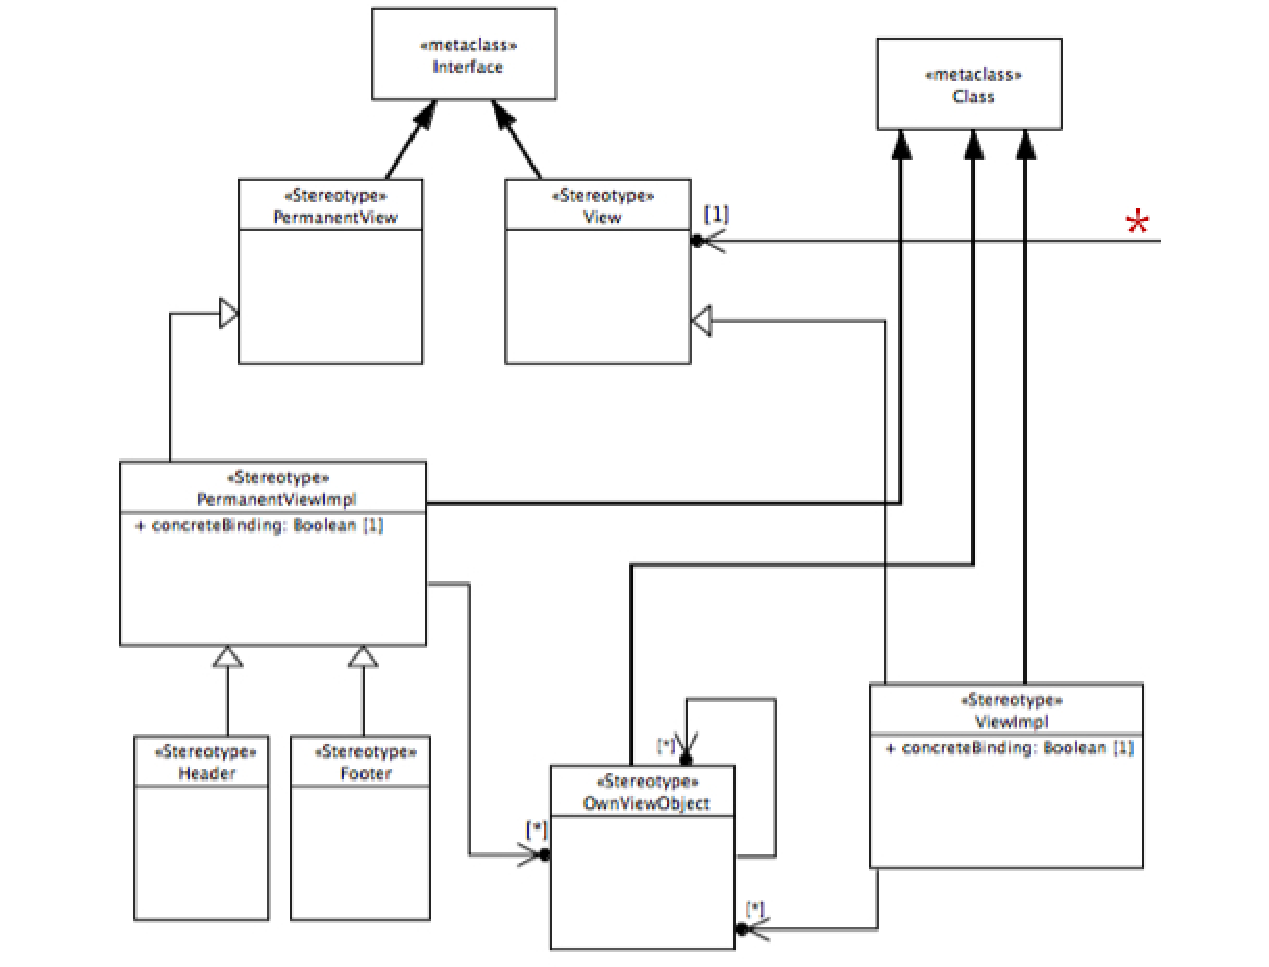
\includegraphics[width=\textwidth]{./img/ProfilClass.pdf}
\caption{Darstellung der Classes und Interfaces im Profil}\label{Fig:UMLProfil}
\end{center}
\end{figure}\\

Es wurden die Stereotypen  \textbf{View} und eine statische  \textbf{PermanentView} von der Metaklasse Interface abgeleitet. Diese bieten eine hilfreiche Schnittstelle für deren Implementationen. Die beiden Interfaces werden als Stereotype  \textbf{ViewImpl} und  \textbf{PermanentViewImpl} der Meta Klasse class implementiert. Durch Erstellen des Boolean - Attributs \textbf{concreteBinding} ist es möglich, den entsprechenden bind-Befehl über den Generator zu setzen. Da im Regelfall kein Interface besteht oder es nur eine Implementierung von einem speziellen Interface gibt, ist dieser Wert per Defaultwert auf true gesetzt. In diesem Fall gib es immer nur diese eine spezielle View, die angezeigt werden kann. Sollte es aber mehrere Implementierungen zu einem Interface geben, muss das  \textbf{concreteBinding}  dieser per Hand angepasst werden. Dadurch wird dieses im Anwendungsfall entsprechend gesetzt und gleichzeitig nur die richtige View ausgewählt.
Anfangs gab es für die Interfaces mehrere Lösungsansätze. In der ersten Fassung beispielsweise erbten auch  \textbf{Footer}  und  \textbf{Header}  direkt vom \textbf{PermanentView} Interface. Da  \textbf{Footer} und  \textbf{Header} aber eigentlich \textbf{PermanentViewImpl} mit vordefinierten, festen Positionen sind, war es sinnvoller diese direkt von der \textbf{PermanentViewImpl} erben zu lassen. So wie es letztendlich in der Endfassung auch umgesetzt wurde.  \\

Für spezielle Klassen wurde noch der Stereotype \textbf{OwnViewObject} hinzugefügt, der es dem Entwickler später ermöglichen soll, als Hülle für mehrere unterschiedliche \textbf{ViewImpl} oder auch \textbf{PermanentViewImpl} zur Verfügung stehen soll. Es dient somit als eigenständiges Widget, das aber die Möglichkeit bietet andere GWT Widgets zu enthalten.

Damit auch hier der Umfang des Arbeitsaufwandes für den GWT Entwickler so gering wie möglich gehalten wird, wurden im Profil die Stereotypen, wie von GWT vorgesehen, Activity und Place nicht angelegt. So müssen sich die Entwickler im M1 Modell zu diesen Klassen keine Gedanken mehr machen, denn mit Hilfe des Generator werden diese automatisch zur entsprechenden View generiert. 
Auch der direkte Stereotype Model, welcher beispielsweise die Schnittstelle zu einer Datenbank repräsentiert hätte, entfällt in dem Profil. Im Projekt war diese Backend-Anbindung nicht vorgesehen. Daten können später direkt in dem UML M1 Modell angegeben werden oder über XML Dateien geladen werden.